
\chapter {Architecture Of Oscad}

“Oscad” is a CAD tool which provides the ease of testing circuits for electronic system designers. But the important feature of this tool is that it is Open Source and hence the user can check,modify the source as per their need. The software provides a generic, modular and extensible platform for experiment with electronic circuits. This software runs on all UNIX platforms and also with python, Kicad, Ngspice and Scilab 5.4 or above.

The objective behind the development of Oscad is to provide an open source solution for electronics and electrical engineers. The software should be capable of performing Circuit Schematic, PCB Design and Circuit Simulation (Analog, Digital and Mix-signal). It should provide facilities to create new models and components. In addition to this, it should have the capability to explain the circuit by giving symbolic equations and numerical values. Keeping these objectives in mind, we have designed the architecture of Oscad.


Keeping the above features in mind, the plan was to
\begin{itemize}
\item Integrate existing open source tools for Circuit Design and drawing, PCB Layout, Circuit Simulation.
\item Create additional modules if required.
\item Create user friendly graphical interface.
\end{itemize} 
%Use this code if you want to include a figure
%\begin{figure}[h]%h stands for 'here'. If h is removed then the fig will go to the bottom or to the next page.
%\begin{center}
%\includegraphics[width=0.2\linewidth]{iitblogo.pdf}%If the fig is appearing too big/small, change the scaling factor 0.2
%\caption{Figure Name}
%\label{iit}
%\end{center}
%\end{figure}
%%%%%%%%%%%%%%%

%pdflatex fileneme.tex
%bibtex  filename.aux
%pdflatex fileneme.tex
%pdflatex fileneme.tex

%Figure \ref{iit} is shown above.

\section {Modules used in Oscad:}
We have used different open-source tools for the underlying build-up of Oscad. In this section we will give a brief idea about all packages. 

\subsection {Eeschema -- Schematic Editor}
Eeschema is an integrated software where all functions of circuit drawing, control, layout, library management and access to the PCB design software are carried out within itself. Eeschema is intended to work with printed circuit software such as Pcbnew. It can provide the netlist file, which describes the electrical connections of the PCB. Eeschema also integrates a component editor which allows the creation, editing and visualization of components. It also allows the user to effectively handle of the symbol libraries i.e; import, export, addition and deletion of library components).

Eeschema also integrates the following additional but essential functions needed for a modern schematic capture software:
\begin{itemize}
\item Design rules check (DRC) for the automatic control of incorrect connections and inputs of components left unconnected.
\item Generation of layout files in POSTSCRIPT or HPGL format.
\item Generation of layout files printable via printer.
\item Bill of Material generation.
\item Netlist generation for PCB layout or for simulation.
\end{itemize}

\subsection {CvPCB -- Component-Footprint mapper}
CvPcb is a tool that allows user to associate components in the schematic to component footprints used when laying out the printed circuit board. Typically the netlist file generated by Eeschema does not specify which printed circuit board footprint is associated with each component in the schematic. Although this is not always the case as component footprints can be associated during schematic capture by setting the component's footprint field. CvPcb provides a convenient method of associating footprints to components. It provides footprint list filtering, footprint viewing, and 3D component model viewing to help ensure the correct footprint is associated to each component. Components can be assigned to their corresponding footprints manually or automatically by creating equivalence files. Equivalence files are look up tables associating each component with it's footprint. This interactive approach is simpler and less error prone than directly associating the footprints in the schematic editor because as well as allowing for automatic association, CvPcb allows you to see the list of available footprints available and display them on the screen to ensure you are associating the correct footprint.

\subsection {Pcbnew -- PCB Layout Editor}
Pcbnew is a powerful printed circuit board software tool. It is used in association with the schematic capture software program Eeschema, which provides the netlist file - this describes the electrical connections of the PCB to design. CvPcb is used to assign each component in the Netlist produced by Eeschema, to a module that is used by Pcbnew.
\begin{itemize}
\item It manages libraries of modules. Each module is a drawing of the physical component including its footprint - the layout of pads providing connections to the component. The required modules are automatically loaded during the reading of the netlist produced by CvPcb.
\item Pcbnew integrates automatically and immediately any circuit modification, by removal of any erroneous tracks, addition of the new components, or by modifying any value (and under certain conditions any reference) of the old or new modules, according to the electrical connections appearing in the scheme.  
\item This tool provides a rats nest display, a hairline connecting the pads of modules which are connected on the schematic. These connections move dynamically as track and module movements are made.
\item It has an active Design Rules Check (DRC) which automatically indicates any error of track layout in real time.
\item It can automatically generates a copper plane, with or without thermal breaks on the pads. 
\item It has a simple but effective autorouter to assist in the production of the circuit. An Export/Import in {\tt SPECCTRA} dsn format allows to use more advanced auto-routers. 
\item This provides options specifically for the production of ultra high frequency circuits (such as pads of trapezoidal and complex form, automatic layout of coils on the printed circuit...). 
\item Pcbnew displays the elements (tracks, pads, texts, drawings and more) as actual size and according to personal preferences:
\begin{itemize}
\item display in full or outline.
\item display of the track/pad clearance.
\end{itemize}
\end{itemize}

\subsection {Kicad to Ngspice netlist converter}
It converts Kicad generated netlists to ngspice compatible format.It has the capability to

\begin{itemize}
\item Insert parameters for fictitious components
\item Convert IC into discrete blocks
\item Insert D-A and A-D converter at appropriate place
\item Insert plotting and printing statement in netlist
\item Find current through all components
\end{itemize}

\subsection {Analysis Inserter}
This feature helps the user to perform different type of analysis such as Operating point analysis, DC analysis, AC analysis, transient analysis etc.It has the facility to

\begin{itemize}
\item Insert type of analysis
\item Option of analysis
\item Option of simulator
\end{itemize}

\subsection {Component Model Builder}
\begin{itemize}
\item This tool provides a facility to define a new model for devices such as 
\begin{itemize}
            \item Diode
            \item Bipolar Junction Transistor (BJT)
            \item Metal Oxide Semiconductor (MOS)
            \item Junction Field Effect Transistor (JFET)
            \item IGBT
            \item Magnetic core
\end{itemize}
\item  Provides facility to edit existing model.
\item  Provides help related to model parameter.
\end{itemize}
 
\subsection{Component Sub-circuit Builder}
This feature allows the user to create a sub-circuit for a component. Once the sub-circuit for a component is created, the user can use it
for different circuits. It has the facility of 
\begin{itemize}
\item Provides facility to define new components such as
\begin{itemize}
\item Op-amp
\item IC-555
\end{itemize}
\item Provides facility to edit existing sub-circuit
\item Provides help related to components parameters
\end{itemize}

\subsection{Circuit Simulator -- Ngspice}
Ngspice is a general-purpose circuit simulation program for nonlinear dc, nonlinear transient, and linear ac analyses. Circuits may contain resistors, capacitors, inductors, mutual inductors, independent voltage and current sources, four types of dependent sources, lossless and lossy transmission lines (two separate implementations), switches, uniform distributed RC lines, and the five most common semiconductor devices: diodes, BJTs, JFETs, MES-FETs, and MOSFETs.
\subsection{Scilab based circuit simulator -- SMCSim}

The feature of SMCSim is that it gives the system of equations for the circuit under test. The SMCSim works in three modes: normal, symbolic and numerical mode. Details about this will be expalined in later chapters.

\section {Workflow of Oscad:}
Fig. 1 shows a block diagram of Oscad\cite{yogesh-paper}. The block diagram consists mainly three parts: 
\begin{itemize}
\item Schematic Editor 
\item PCB Layout Editor  
\item Circuit Simulators
\end{itemize} 


%Use this code if you want to include a figure
%Use this code if you want to include a figure
\begin{figure}[h]%h stands for 'here'. If h is removed then the fig will go to the bottom or to the next page.
\begin{center}
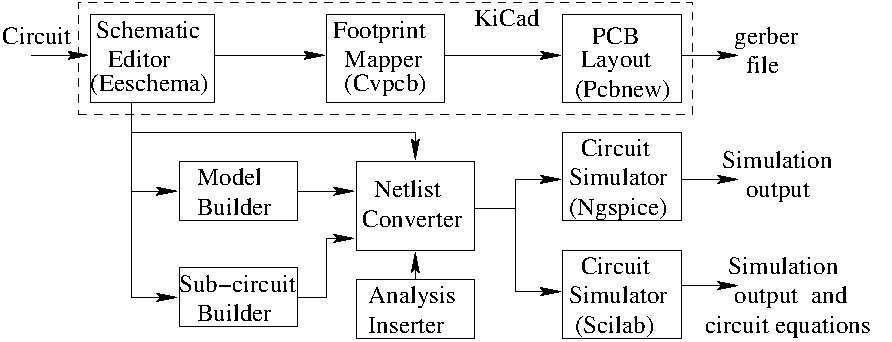
\includegraphics[width=1\linewidth]{figures/oscadBD-eps-converted-to.pdf}%If the fig is appearing too big/small, change the scaling factor 0.2
\caption{Block Diagram of Oscad}
\label{iit}
\end{center}
\end{figure}
%%%%%%%%%%%%%%%
Here, we explain the functionality of each block to design electronic systems.

The circuit design is the first step of design of an electronic circuit. Generally a circuit diagram is drawn on a paper, and then entered into a computer using a schematic editor. We have used Eeschema as a schematic editor for Oscad. Thus all the functionalities of Eeschema are naturally available in Oscad.

Using the functionalities of Eeschema, we have created separate libraries for components supported by ngspice ex-plicitly or implicitly. As Eeschema is originally intended for PCB Design, there are no fictitious components5 such as voltage or current sources. Thus, we have added a new library for different types of voltage and current sources such as sine, pulse, square wave, etc. We have also built a library
which gives a functionality of printing and plotting solution.

The schematic editor provides a netlist file, which describes the electrical connections of the PCB to a design. In order to create a PCB layout, physical components are required to map into their footprints. To create component to footprint mapping, we have used Cvpcb software which is a part of KiCad . For additional components in newly defined library, we have assigned or created footprints. We have used Pcbnew software to draw a PCB layout.


After designing a circuit, it is essential to check the integrity of the circuit design. In case of large size electronic circuits, breadboard testing is impractical. Therefore electronic system designers rely heavily on simulation.


The accuracy of the simulation results can be increased by accurate modeling of the circuit elements. Model Builder, provides a facility to define a new model for devices and edit existing models. Complex circuit elements can be created by hierarchical modeling. Sub-circuit Builder provides an easy way to create a sub-circuit. The schematic editor provides a netlist file, which describes the electrical connections between circuit components. But it cannot be directly used for simulation due to compatibility issues. Netlist Converter, denoted converts the netlist into a Ngspice compatible netlist. The type of simulation to be performed using the netlist and the corresponding options are provided through a graphical user interface (GUI). We call this as the Analysis Inserter.


We have used Ngspice for mixed-level/mixed-signal circuit simulation. Ngspice is based on three open source software packages\cite{spice}: 
\begin{itemize}
\item Spice3f5 (analog circuit simulator) 
\item Cider1b1 (couples Spice3f5 circuit simulator to DSIM device simulator)
\item Xspice (code modeling support and simulation of digital components through an event driven algorithm)
\end{itemize}
 
It is a part of gEDA project. Ngspice is capable of simulating devices with BSIM, EKV, HICUM, HiSim, PSP, PTM models. It is widely used due to its accuracy even for latest technology devices.

In order to provide an explanation capability, we have also developed a Scilab based circuit simulation capability within OSCAD. It generates equations from the netlist and gets them solved by Scilab, which has many state of the art numerical methods built in. We have referred to this as Scilab based Mini Circuit Simulator (SMCSim).








